\documentclass[parskip=full]{scrartcl}
\usepackage{graphicx, graphbox, subcaption}
\usepackage{hyperref}
\graphicspath{ {../screenshots} }
\begin{document}
\begin{titlepage}
\title{Exploration and Presentation Assignment 3}
\subtitle{Optimization}
\author{Simon Schønberg Bojesen - cph-sb339@cphbusiness.dk
    \and Kenneth Hansen- cph-kh415@cphbusiness.dk
    \and Frederik Blem - cph-fb114@cphbusiness.dk
    \and Martin Høigaard Cupello - cph-mr221@cphbusiness.dk}
\maketitle
\thispagestyle{empty}
\end{titlepage}
\clearpage

\section{Introduction}
\label{sec:introduction} % Don't use bold this way in the actual report - only for template purpose.
    We chose to optimize the program \href{https://github.com/CPHBusinessSoftUFO/letterfrequencies}{letterfrequencies}.
    This program opens any textfile and counts all instances of each letter occuring in textfile, and prints the results. We had as assignment to optimize the programs performance by at least 50\%.
\clearpage

\section{Documentation of the current performance}
\label{sec:currentdoc} 
    First we needed to document the current performance to be able to show how the current program performed. To do that we had to add a Timer class to time the programs runtime.

\begin{figure}[!h]
    \captionabove{Timer.java}
    \centering
    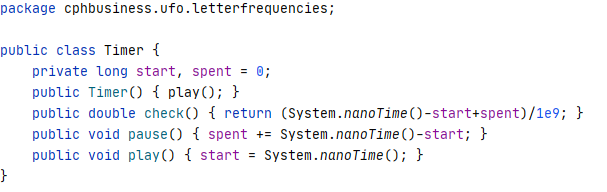
\includegraphics[width=\textwidth]{Timer.PNG}
\end{figure}


\begin{figure}[!h]
    \captionabove{Main.java}
    \centering
    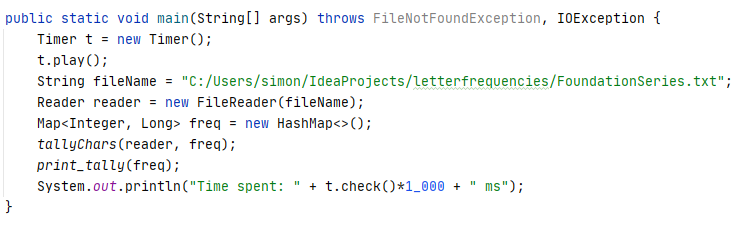
\includegraphics[width=\textwidth]{unchanged_code_added_timer.png}
\end{figure}

After making these changes each person in our group ran 10 individual speedtests of the program on their systems.
These test results were then put in our own named files in the testnotes folder.
We then made a boxplot showing the results of our tests, and calculated the means. 
From these means we calculated the goal performances each of our systems needed to reach by optimization.
\clearpage

\begin{figure}
    \captionabove{Boxplot of all test results} % Caption on top of both of the images.
    \centering % Centering requirement met
    \begin{subfigure}[b]{0.4\textwidth}
        \caption{Simon's tests.} 
        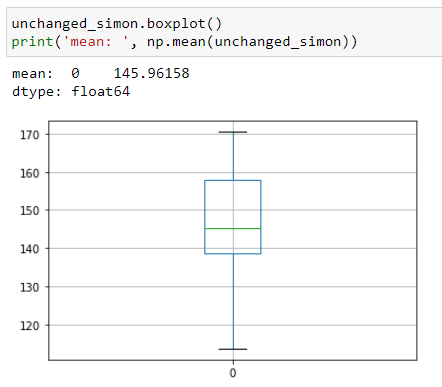
\includegraphics[width=\textwidth]{simon_unchanged.PNG}
    \end{subfigure}
    \begin{subfigure}[b]{0.4\textwidth}
        \caption{Frederik's tests.} 
        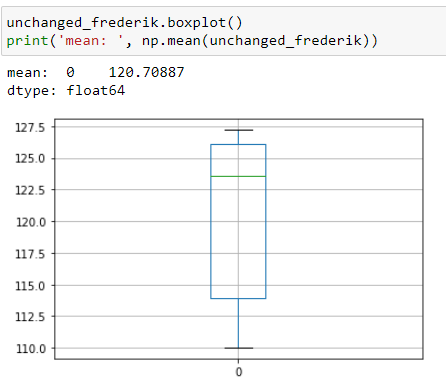
\includegraphics[width=\textwidth]{frederik_unchanged.PNG}
    \end{subfigure}
    \begin{subfigure}[b]{0.4\textwidth}
        \caption{Martin's tests.}
        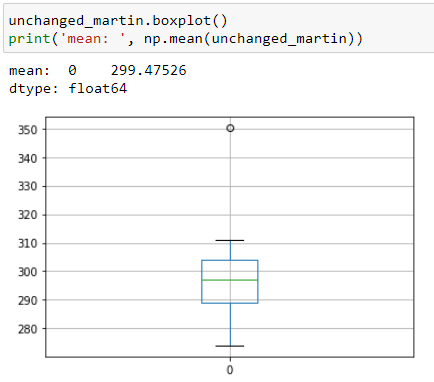
\includegraphics[width=\textwidth]{martin_unchanged.PNG}
    \end{subfigure}
    \begin{subfigure}[b]{0.4\textwidth}
        \caption{Kenneth's tests.} 
        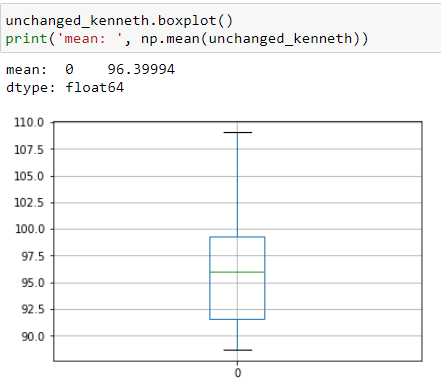
\includegraphics[width=\textwidth]{kenneth_unchanged.PNG}
    \end{subfigure}
  \end{figure}

As we can see our systems performance varied greatly. We then calculated minimum goals for each of us from these means.
The goal is to increase performance as measured by time.

Simon mean: 145.96158\\
Frederik mean: 120.70887\\
Martin mean: 299.47526\\
Kenneth mean: 96.39994

These numbers needs to be reduced by 50\% as per the assignment.
We have calculated the goal means to be:

Simon: 108.75\\
Frederik: 90.5316525\\
Martin: 224.606445\\
Kenneth: 72.299955
\clearpage

\section{Bottlenecks and hypothesis of issues}
\subsection{Finding bottlenecks}
First thing we needed to do was figuring out what method would give us better performance by optimization.
Therefore we ran the program in IntelliJ Ultimate, with a profiler to see which methods were the most expensive.

\begin{figure}[!h]
    \captionabove{Profiler Flame Chart}
    \centering
    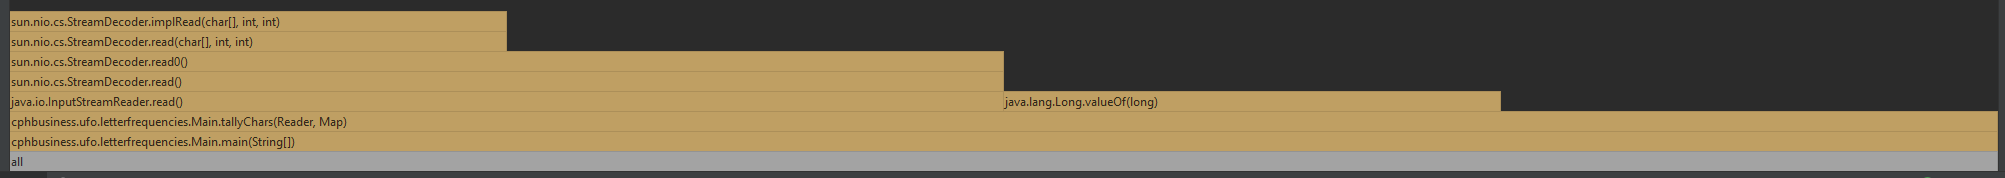
\includegraphics[width=\textwidth]{unchanged_code_flame_graph.png}
\end{figure}

\begin{figure}[!h]
    \captionabove{Profiler Call Tree}
    \centering
    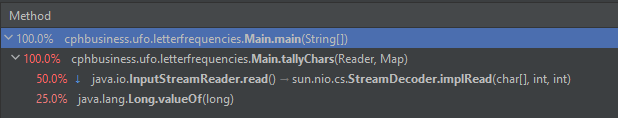
\includegraphics[width=\textwidth]{unchanged_code_call_tree.png}
\end{figure}

These charts clearly state that all of the costly functionality is in the method tallyChars. 
We then moved the timer around to check how fast the other function: "print\_tally" was as this method was not showing up in our profiler. 
It averaged at about 5 ms for simon, and we therefore concluded it wasnt worth optimizing.
\clearpage
\subsection{Why is tallyChars so expensive}
As we looked at he profiler it was quite clear to us that we needed to improve the speed of reading the file.
After searching google, we figured out using a BufferedReader instead might be the way to go.

\begin{figure}[!h]
    \captionabove{Changed Reader Type}
    \centering
    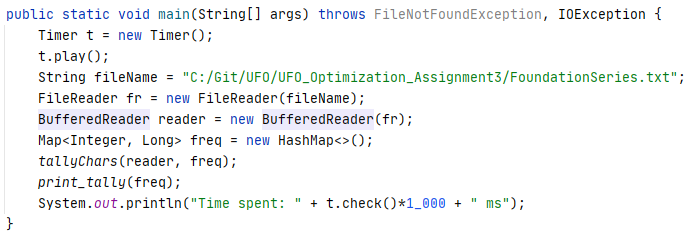
\includegraphics[width=\textwidth]{changed_code2.PNG}
\end{figure}

\begin{figure}[!h]
    \captionabove{Changed tallyChars Arguments}
    \centering
    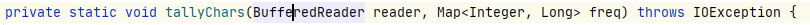
\includegraphics[width=\textwidth]{changed_code1.PNG}
\end{figure}

After this one change we saw significant change to the performance, and decided to make samples and check if we hit our goals.
\clearpage

\section{Documentation of performance after optimization}
\begin{figure}[!hb]
    \captionabove{Boxplot of optimized test results} % Caption on top of both of the images.
    \centering % Centering requirement met
    \begin{subfigure}[b]{0.35\textwidth}
        \caption{Simon's tests.} 
        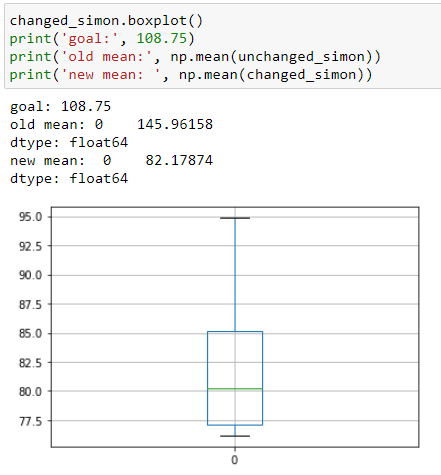
\includegraphics[width=\textwidth]{simon_changed.PNG}
    \end{subfigure}
    \begin{subfigure}[b]{0.35\textwidth}
        \caption{Frederik's tests.} 
        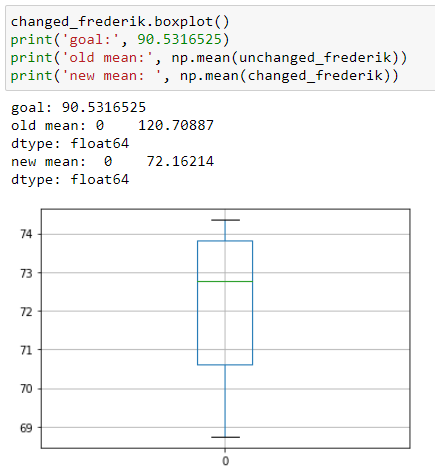
\includegraphics[width=\textwidth]{frederik_changed.PNG}
    \end{subfigure}
    \begin{subfigure}[b]{0.35\textwidth}
        \caption{Martin's tests.}
        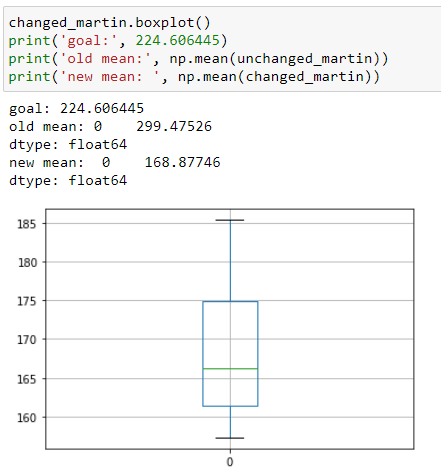
\includegraphics[width=\textwidth]{martin_changed.PNG}
    \end{subfigure}
    \begin{subfigure}[b]{0.35\textwidth}
        \caption{Kenneth's tests.} 
        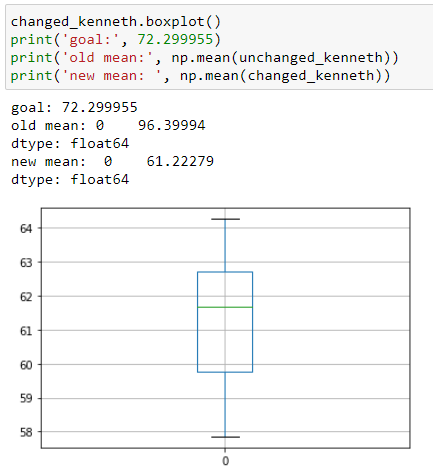
\includegraphics[width=\textwidth]{kenneth_changed.PNG}
    \end{subfigure}
  \end{figure}

We accomplished our goals on that one optimization and were even very close to the 100\% improvement stated in the assignment as possible. We therefore concluded the project here.
\end{document}


